\documentclass[10pt,times]{beamer}
\usepackage{amsfonts}
\usepackage{amsmath}
\usepackage{amssymb}
\usepackage{mathptmx}

\usepackage{color}
\usepackage{minted}
\usepackage{hyperref}
\usepackage{multicol}
\usepackage{tabularx}
\usepackage{booktabs}
\usepackage{menukeys}

% Stolen from John Miller's LaTeX course
\newcommand{\bftt}[1]{\textbf{\texttt{#1}}}
\newcommand{\comment}[1]{{\color[HTML]{008080}\textit{\textbf{\texttt{#1}}}}}
\newcommand{\cmmd}[1]{{\color[HTML]{008000}\bftt{#1}}}
\newcommand{\bs}{$\backslash$}
\newcommand{\cmdbs}[1]{\cmmd{\bs#1}}
\newcommand{\lb}{{\char'173}}% Left brackets -> {
\newcommand{\rb}{{\char'175}}% Right brackets -> }
\newcommand{\cmdbegin}[1]{\cmdbs{begin\lb}\bftt{#1}\cmmd{\rb}}
\newcommand{\cmdend}[1]{\cmdbs{end\lb}\bftt{#1}\cmmd{\rb}}



% this is where the example source files are loaded from
% do not include a trailing slash
\newcommand{\wllogo}{\textbf{Overleaf}}
\newcommand{\fileuri}{https://raw.githubusercontent.com/kks32/latex-course/master/exercises/}
\newcommand{\wlserver}{https://www.overleaf.com}
\newcommand{\wlnewdoc}[1]{\wlserver/docs?snip\_uri=\fileuri#1\&splash=none}

\def\tikzname{Ti\emph{k}Z}


% stolen from minted.dtx
\newenvironment{exampletwoup}
  {\VerbatimEnvironment
   \begin{VerbatimOut}{example.out}}
  {\end{VerbatimOut}
   \setlength{\parindent}{0pt}
   \fbox{\begin{tabular}{l| l}
   \begin{minipage}{0.55\linewidth}
     \inputminted[fontsize=\small,resetmargins]{latex}{example.out}
   \end{minipage} &
   \begin{minipage}{0.35\linewidth}
     \input{example.out}
   \end{minipage}
   \end{tabular}}}

\newenvironment{exampletwouptiny}
  {\VerbatimEnvironment
   \begin{VerbatimOut}{example.out}}
  {\end{VerbatimOut}
   \setlength{\parindent}{0pt}
   \fbox{\begin{tabular}{l|l}
   \begin{minipage}{0.55\linewidth}
     \inputminted[fontsize=\scriptsize,resetmargins]{latex}{example.out}
   \end{minipage} &
   \begin{minipage}{0.35\linewidth}
     \setlength{\parskip}{6pt plus 1pt minus 1pt}%
     \raggedright\scriptsize\input{example.out}
   \end{minipage}
   \end{tabular}}}

% ******************************** Meta-data ***********************************
\mode<presentation>
{
  \usetheme{Madrid}
  \setbeamercovered{transparent}
}


\usepackage{caption}
\captionsetup{font=scriptsize, labelfont=scriptsize, justification=centering}

\title{Writing papers and thesis using \LaTeX2e}

\author {Krishna Kumar \inst{*}\thanks{kks32@cam.ac.uk} }

\institute[ University of Cambridge ] % (optional, but mostly needed)
{
  \inst{1}%
  King's College\\
  University of Cambridge
}

\date[LaTeX course 2014] % (optional, should be abbreviation of conference name)
{\LaTeX for Beginners}


% Delete this, if you do not want the table of contents to pop up at
% the beginning of each subsection:
%\AtBeginSubsection[]
%{
%  \begin{frame}<beamer>{Outline}
%    \tableofcontents[currentsection,currentsubsection]
%  \end{frame}
%}


% If you wish to uncover everything in a step-wise fashion, uncomment
% the following command: 

% \beamerdefaultoverlayspecification{<+->}

\subtitle{Part I: Introduction to \LaTeX}
%***************************** Title page **************************************
\begin{document}
\begin{frame}
  \titlepage
\end{frame}
%*******************************************************************************
%**************************** Introduction *************************************
%*******************************************************************************
\section{Introduction to \LaTeX2e}

%*******************************************************************************
%******************************* Frame *****************************************
%*******************************************************************************
\begin{frame}{What is \LaTeX?}
\begin{itemize}
\item \LaTeX is a document preparation system for the \TeX typesetting 
program. 

\item Programmable desktop publishing, which automates most of the typesetting.

\item \LaTeX produce beautiful documents, especially mathematics
\begin{equation*}
i \hbar \frac{\partial}{\partial t} \Psi(r,t) = 
\left[\frac{-\hbar^2}{2\mu}\nabla^2+V(r,t)\right]\Psi(r,t)
\end{equation*}

\begin{equation*}
E^2 = (pc)^2 + (m_0 c^2)^2
\end{equation*}

\item \LaTeX is WYSIWYM (What You See is What You Mean)

\end{itemize}
\end{frame}

%*******************************************************************************
%******************************* Frame *****************************************
%*******************************************************************************
\begin{frame}{Can you see beyond the WYSIWYG bubble?}
\begin{figure}
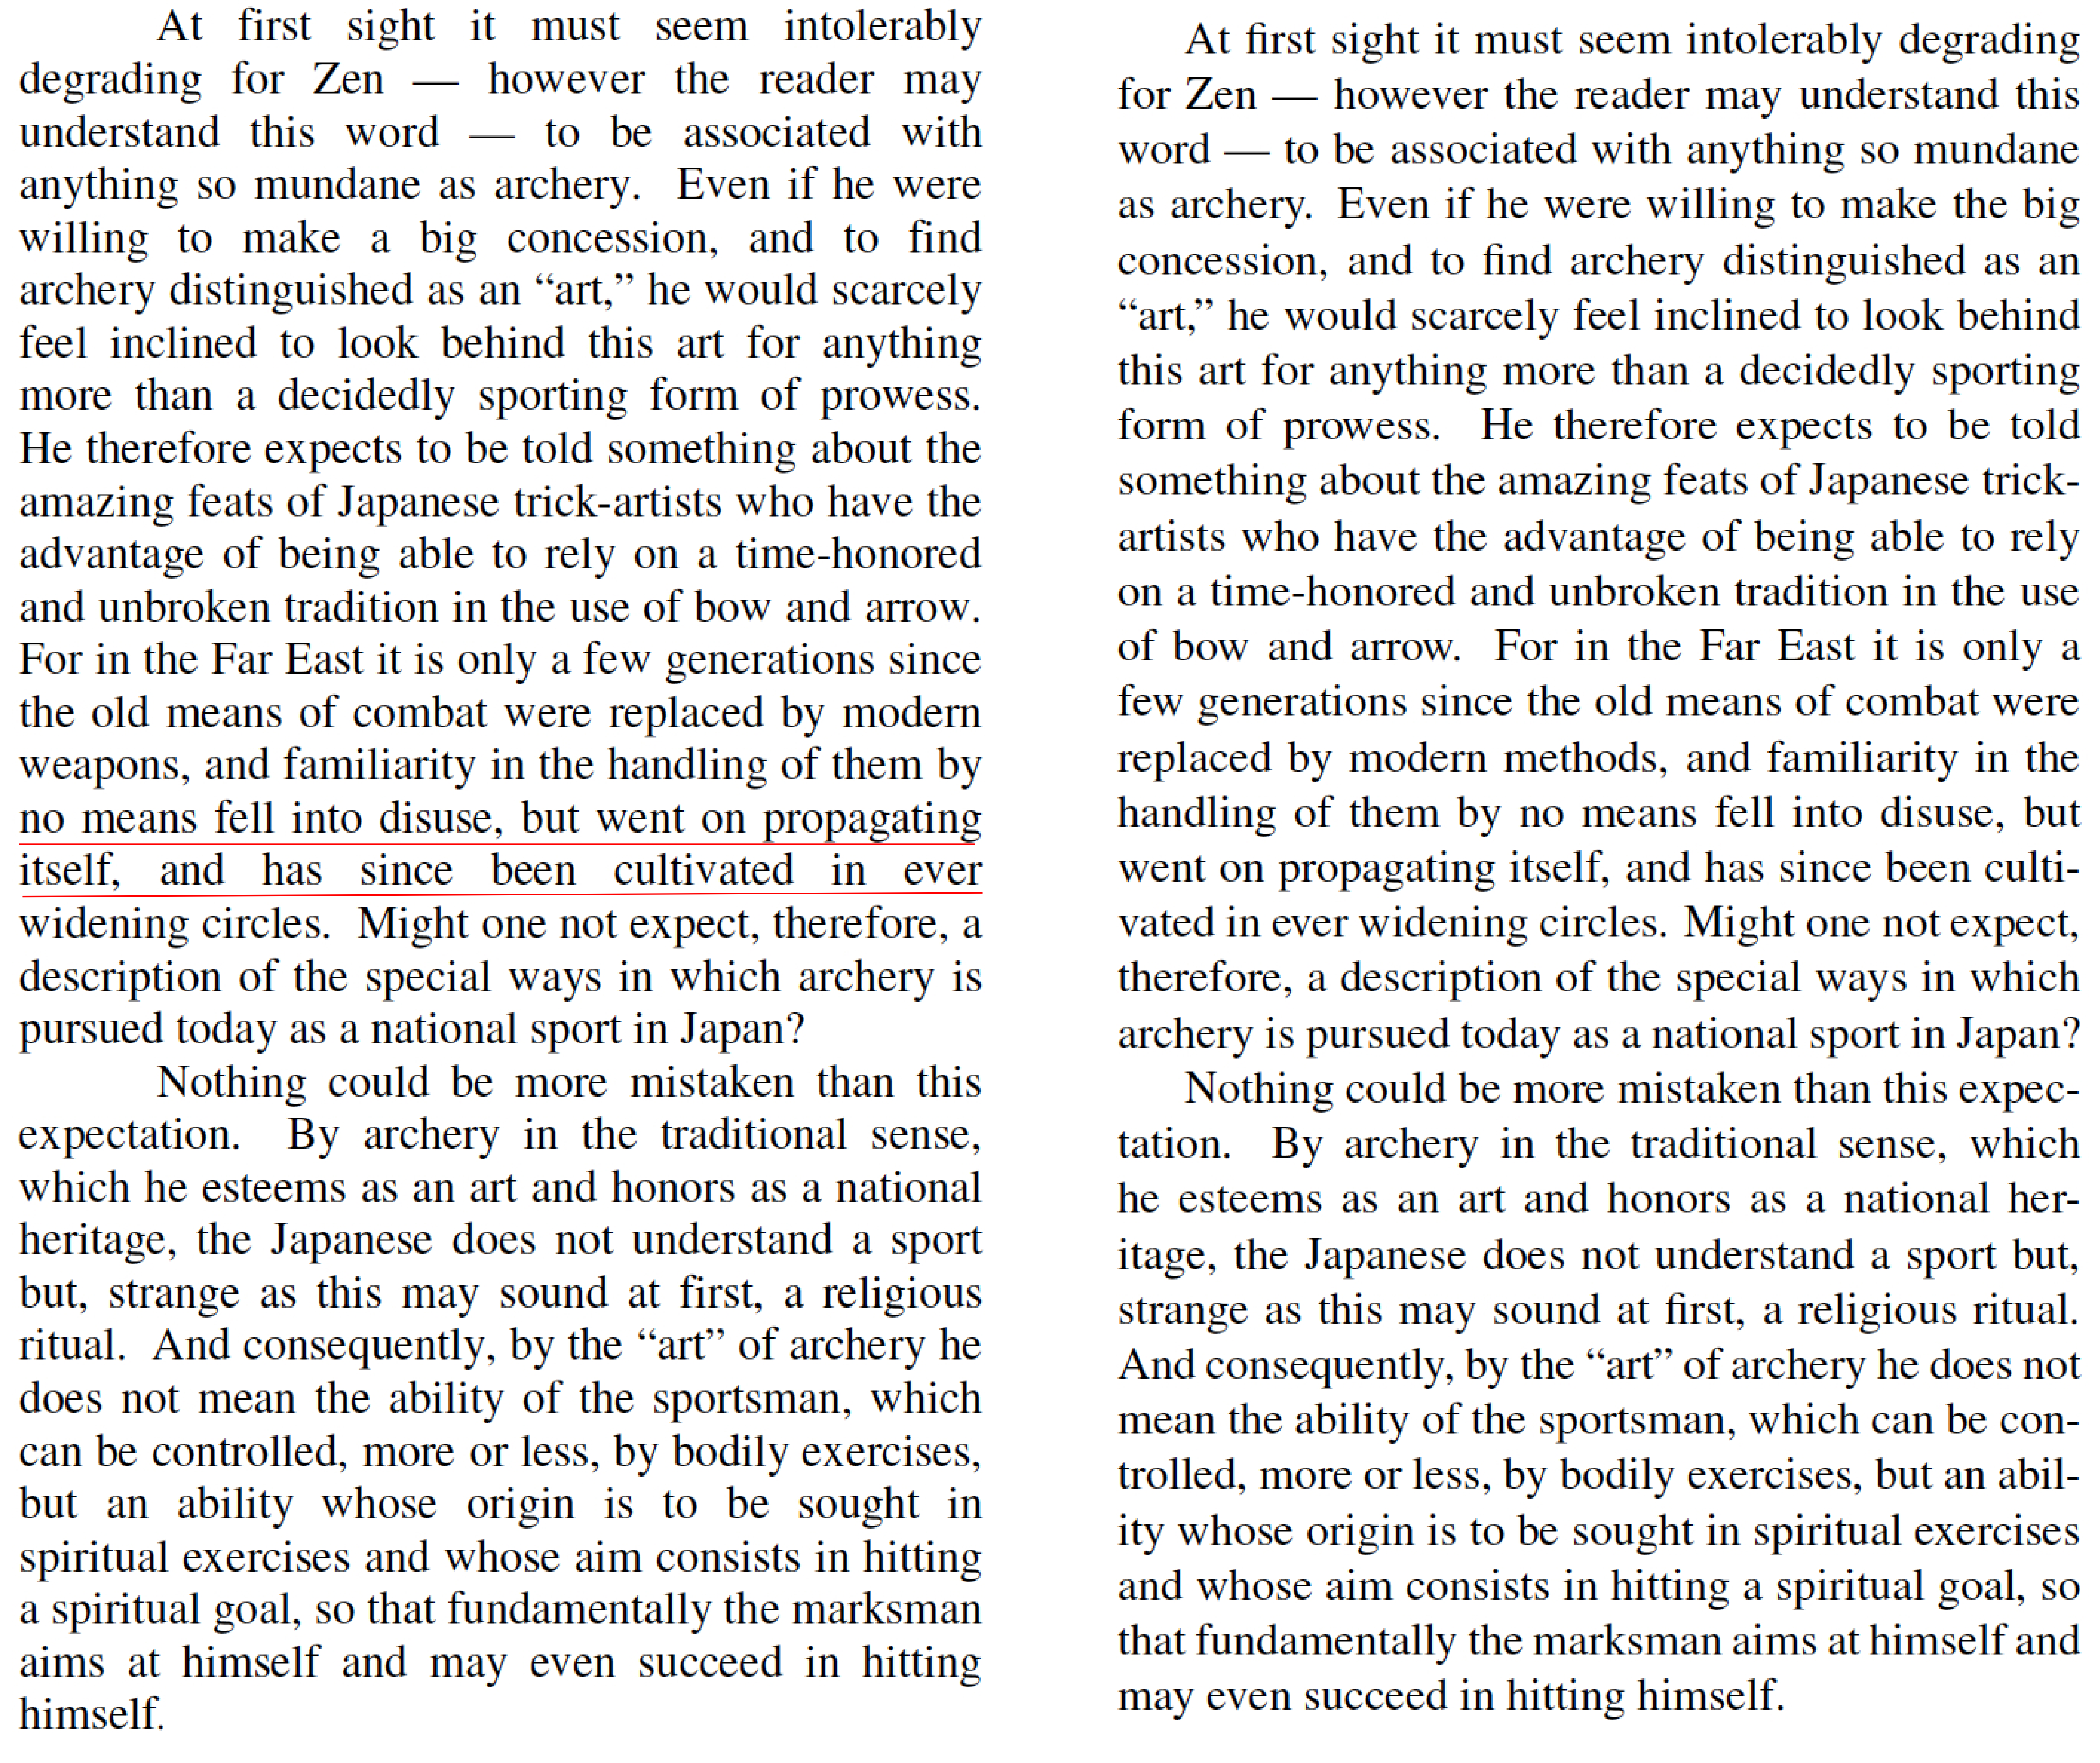
\includegraphics[height=0.85\textheight]{figs/LaTeX_Word.png}
\end{figure}
\end{frame}

%*******************************************************************************
%******************************* Frame *****************************************
%*******************************************************************************
\begin{frame}{Ligatures}
\begin{figure}
\centering

\includegraphics[width=0.7\textwidth]{figs/ligatures_word.png}
\caption{MS Word}
\end{figure}
\begin{figure}
\centering

\includegraphics[width=0.7\textwidth]{figs/ligatures_latex.png}
\caption{\LaTeX}
\end{figure}
\flushright
D.Taraborelli (2008), The Beauty of \LaTeX
\end{frame}

%*******************************************************************************
%******************************* Frame *****************************************
%*******************************************************************************
\begin{frame}
\frametitle{Developers}
\begin{itemize}
\item
\parbox{0.25\textwidth}{
	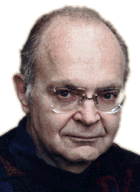
\includegraphics[width=0.15\textwidth]{figs/Donald_Knuth.png}}
\parbox{0.65\textwidth}{Donald Knuth, 1977, \TeX ~Version 3.141592}
\item
\parbox{0.25\textwidth}{
	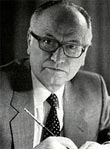
\includegraphics[width=0.15\textwidth]{figs/Hermann.jpg}}
\parbox{0.65\textwidth}{Hermann Zapf}
\item
\parbox{0.25\textwidth}{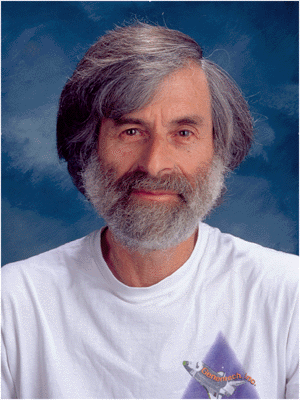
\includegraphics[width=0.15\textwidth]{figs/Leslie.png}}
\parbox{0.65\textwidth}{Leslie Lamport, \LaTeX2e}
\end{itemize}
\end{frame}

%*******************************************************************************
%******************************* Frame *****************************************
%*******************************************************************************
\begin{frame}{How \LaTeX works? - The Magic}
\begin{itemize}
\item You write your document in \texttt{plain text} with \cmd{commands} that
describe its structure and meaning.
\item The \LaTeX program processes your text and commands to produce a
beautifully formatted document.
\end{itemize}

\centering
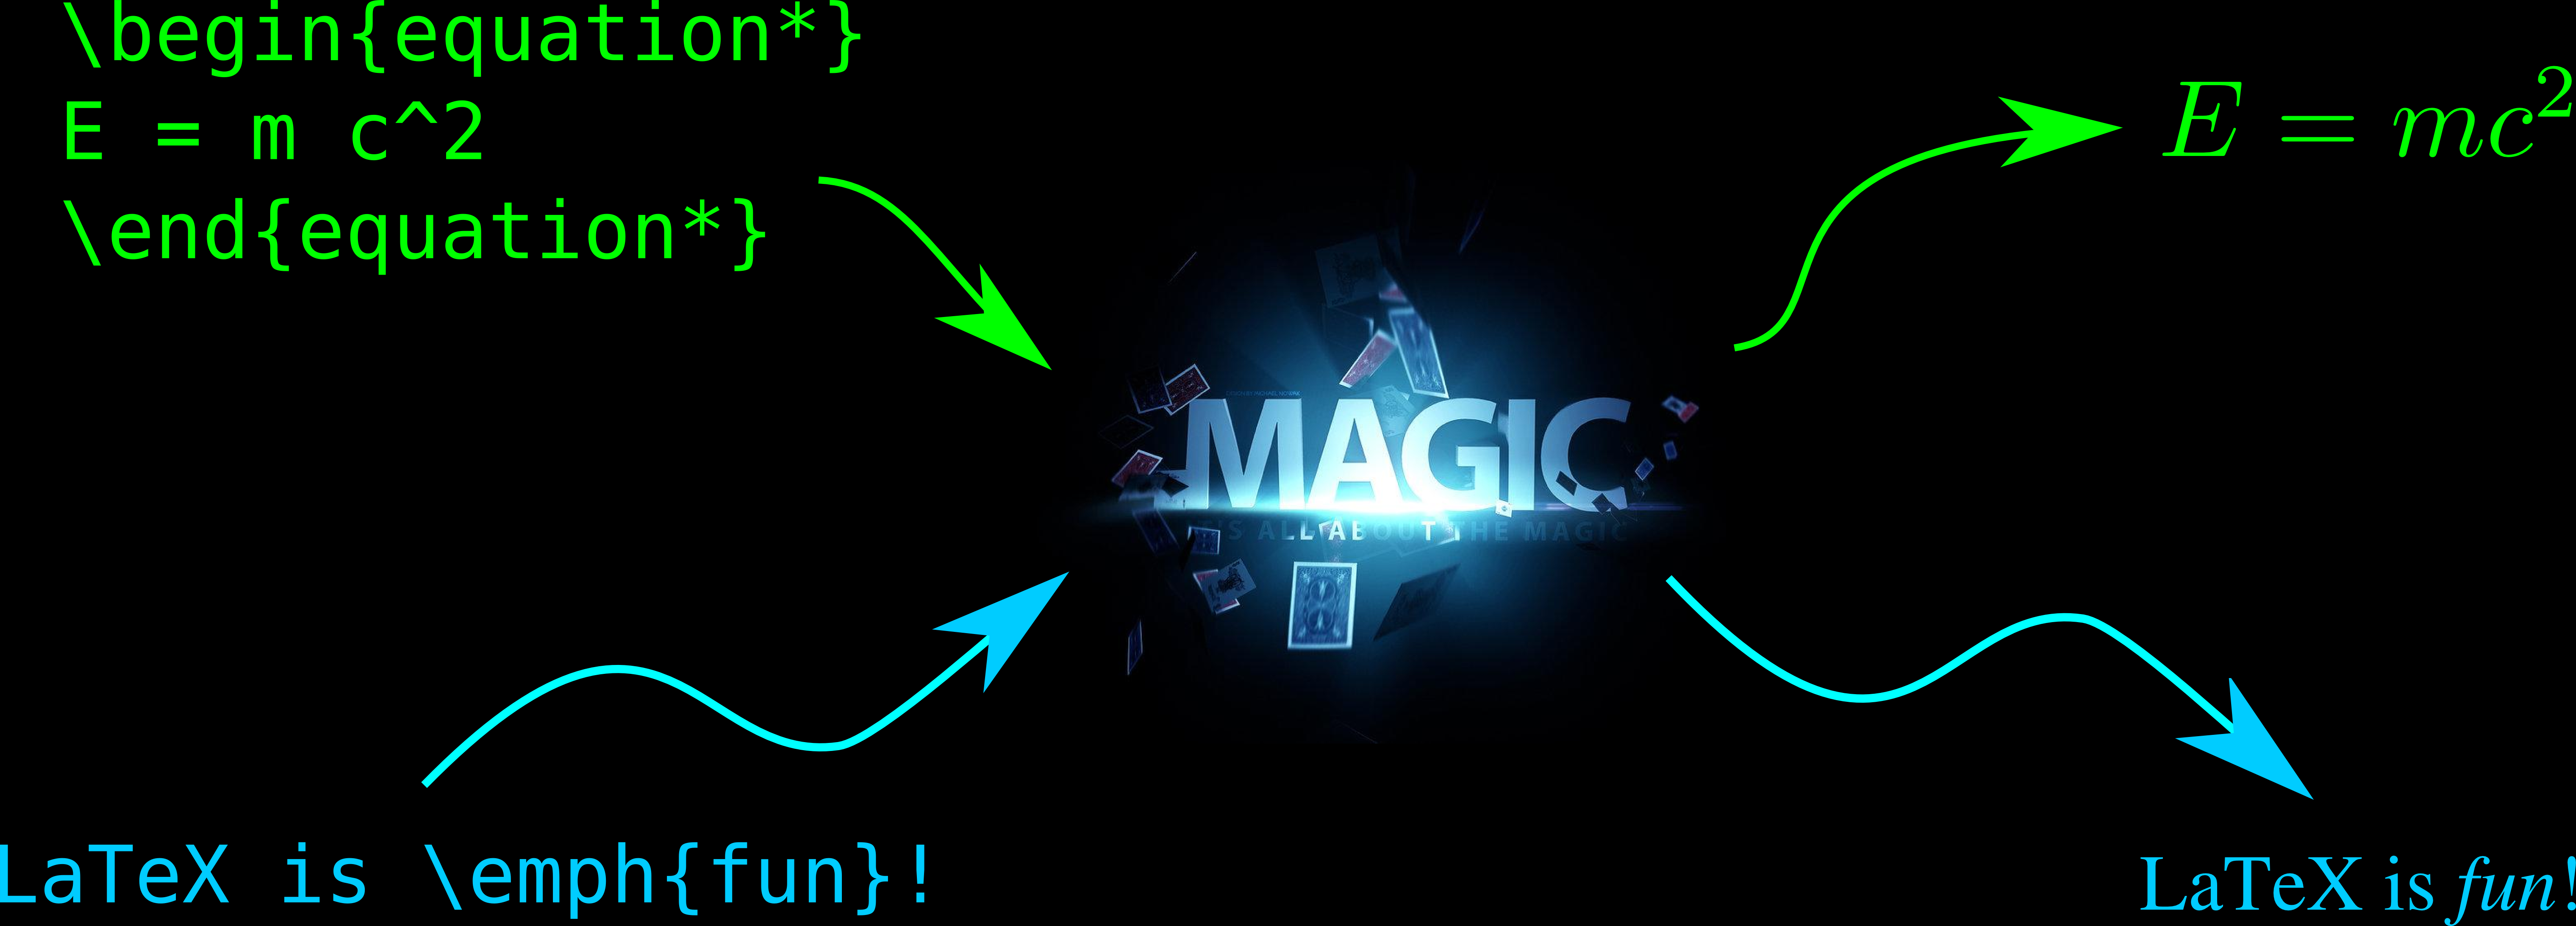
\includegraphics[width=0.95\textwidth]{figs/magic.png}
\end{frame}



%******************************* Frame *****************************************
\begin{frame}{\LaTeX Pros and Cons}
\textbf{Pros}
\begin{itemize}
\item    It's free and works on Macs, Windows, Unix/Linux.
\item    LaTeX files are ASCII and are portable.
\item    The typesetting is better, especially the maths.
\item    Style changes are neater in LaTeX. 
\end{itemize}
\textbf{Cons}
\begin{itemize}
\item    Special/Modern Font selection is difficult, but one can use XeTeX.
\item    LaTeX encourages (almost insists on) structured writing and the 
separation of style from content. This is not the way that many people 
(especially non-programmers) are used to working.
\item    Without a WYSIWYG front end, it's not always easy to find out how to 
do things.
\end{itemize}
\end{frame}



%******************************* Frame *****************************************
\section{Structure}

%******************************* Frame *****************************************

\begin{frame}{LaTeX Structure}
\begin{figure}
\centering
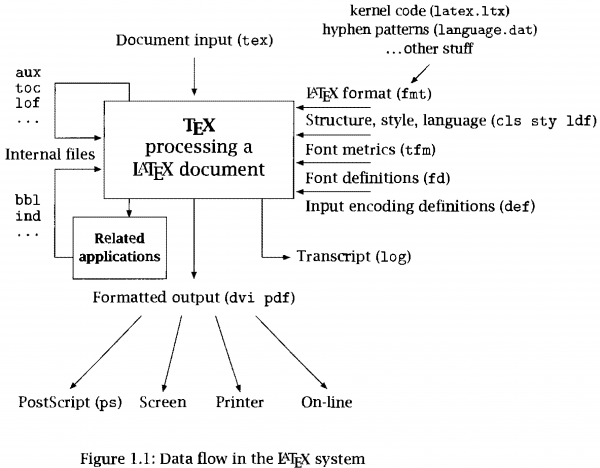
\includegraphics[width=0.7\textwidth]{figs/LaTeX.png}
\end{figure}
\end{frame}


%******************************* Frame *****************************************
\begin{frame}{$\backslash$documentclass\{\}}

\begin{table}
\begin{tabular}{|l|p{0.75\textwidth}|}
\hline
article & articles in scientific journals, presentations, short reports, program documentation, invitations, \dots \\ \hline
IEEEtran & IEEE Transactions format.\\ \hline
proc & A class for proceedings based on the article class.\\ \hline
minimal & Is as small as it can get. It only sets a page size and a base font. It is mainly used for debugging purposes.\\ \hline
report & For longer reports containing several chapters, small books, thesis, \dots \\ \hline
book & For real books.\\ \hline
slides & For slides. The class uses big sans serif letters.\\ \hline
memoir & For changing sensibly the output of the document. It is based on the book class, but you can create any kind of document with it\\ \hline
letter & For writing letters. \\ \hline
beamer& For writing presentations \\ \hline
\end{tabular}
\end{table}
\end{frame}


%**********************************************FRAME***************************************
\begin{frame}{Article, Report and Book}
\begin{table}
\begin{tabular}{|l|c|l|c|}
\hline
\multicolumn{2}{c}{\textbf{Article}}  & \multicolumn{2}{c}{\textbf{report}} \\ 
\hline
\textbf{section} &\textbf{ numbering} & \textbf{section} & \textbf{numbering} \\ \hline
$\backslash$part & 0 & $\backslash$part & -1 \\ \hline
$\backslash$chapter & 0 & $\backslash$section & 1 \\ \hline
$\backslash$section & 1 & $\backslash$subsection & 2 \\ \hline
$\backslash$subsection & 2 & $\backslash$subsubsection & 3 \\ \hline
$\backslash$subsubsection & 3 & $\backslash$paragraph & 4 \\ \hline
$\backslash$paragraph & 4 & $\backslash$subparagraph & 5 \\ \hline
$\backslash$subparagraph & 5 & & \\ \hline

\end{tabular}
\end{table}
\end{frame}

%**********************************************FRAME***************************************
\begin{frame}{$\backslash$documentclass$[$\textbf{options}$]$\{\}}
\begin{table}
\begin{tabular}{|p{0.15\textwidth}|p{0.65\textwidth}|}
\hline
Xpt & Sets the size of the main font in the document. Default: 10pt. \\
a4paper, \newline letterpaper & Defines the paper size. Default: letter/A4. \\
fleqn & displays formulas left-aligned instead of centered. \\
leqno & Places the numbering of formulas on the left hand side instead of the right. \\
titlepage,\newline  notitlepage & Specifies whether a new page should be started after the document title or not. The article class does not start a new page by default, while report and book do.\\
onecolumn,\newline  twocolumn & Instructs LaTeX to typeset the document in one column or two columns. \\
\end{tabular}
\end{table}
\end{frame}


%**********************************************FRAME***************************************

\begin{frame}{$\backslash$documentclass$[$\textbf{options}$]$\{\} cont \dots}
\begin{table}
\begin{tabular}{|p{0.15\textwidth}|p{0.65\textwidth}|}
twoside,\newline  oneside & double or single sided output. Article and report are single sided and the book is double sided by default. \\
landscape & Changes the layout of the document to print in landscape mode. \\
openright,\newline  openany & Makes chapters begin either only on right hand pages or on the next page available. This does not work with the article class, as it does not know about chapters. \\
draft & Draft - no images. \\
\end{tabular}
\end{table}
\end{frame}


%**********************************************FRAME***************************************
\begin{frame}{Fonts}
\begin{itemize}
\item \tiny $\backslash$tiny
\item \scriptsize $\backslash$scriptsize
\item \footnotesize $\backslash$footnotesize
\item \small $\backslash$small
\item \normalsize $\backslash$normalsize
\item \large $\backslash$large
\item \Large $\backslash$Large
\item \LARGE $\backslash$LARGE
\item \huge $\backslash$huge
\item \Huge $\backslash$Huge
\end{itemize}
\end{frame}


%**********************************************FRAME***************************************

\begin{frame}{Restricted Characters}
\begin{table}
\begin{tabular}{cc}
\hline
\textbf{Character} & \textbf{How to type in LaTeX} \\  \hline
\# & $\backslash$\# \\ 
\& & $\backslash$\& \\ 
\$ & $\backslash$\$ \\
\% & $\backslash$\% \\ 
$\backslash$ & \$$\backslash$backslash\$ \\ 
\_ & $\backslash$\_ \\
\{ & $\backslash$\{ \\
\} & $\backslash$\} \\

\end{tabular}
\end{table}
\end{frame}


%**********************************************FRAME***************************************


%**********************************************FRAME***************************************
\begin{frame}{Equations}
The Energy-Momentum Relation: $E^2 = (m_0c^2)^2 + (pc)^2$ \\
\begin{equation}
 f(x)= \sin^2x+\frac{\tan \mathit{x}}{\log \mathit{x}} + \mathbf{X}^T\times\mathbf{X}
\end{equation}

\begin{equation*}
\iint_{0}^{\infty}   f(x,y)dx dy
\end{equation*}

\begin{eqnarray}
	y   & = & ax+b \nonumber\\
	y+1 & = & ax+(b+1)\\
	    & = & ax+(b+2)-1
\end{eqnarray}

\end{frame}

%**********************************************FRAME***************************************
\begin{frame}{Equations cont\dots}

\begin{multline}
f(x)=a1x_1+a2x_2+a3x_3+a_4x_4+
\sqrt{a1x_1+a2x_2+a3x_3+a_4x_4}+\\
a1x_1+a2x_2+a3x_3+a_4x_4+
a1x_1+a2x_2+a3x_3+a_4x_4
\end{multline}

\begin{equation}
A_{m,n} =
 \begin{pmatrix}
  a_{1,1} & a_{1,2} & \cdots & a_{1,n} \\
  a_{2,1} & a_{2,2} & \cdots & a_{2,n} \\
  \vdots  & \vdots  & \ddots & \vdots  \\
  a_{m,1} & a_{m,2} & \cdots & a_{m,n}
 \end{pmatrix}
\end{equation}
\end{frame}

%**********************************************FRAME***************************************
\begin{frame}{Matrix}
\begin{center}
\begin{tabular}{l c}
\textbf{Environment name} &	\textbf{Surrounding delimiter} \\
pmatrix	& $( matrix )$  \\
bmatrix	&	$[ matrix ]$  \\
Bmatrix	&	$\{ matrix \}$ \\
vmatrix	&	$| matrix |$ \\
Vmatrix &	$|| matrix ||$  \\
\end{tabular}
\end{center}
\end{frame}

%**********************************************FRAME***************************************
\section{Tables}
%**********************************************FRAME***************************************
\begin{frame}{Table Environment}

\begin{table}
\begin{tabular}{ll} \hline
\textbf{Option} & \textbf{Description} \\ \hline
l  &	left-justified column \\
c  &	centered column  \\
r  &	right-justified column  \\
p\{`width'\} &	paragraph column with text vertically aligned at the top  \\
m\{`width'\} & 	paragraph column with text vertically aligned in the middle \\
b\{`width'\} &	paragraph column with text vertically aligned at the bottom  \\
| &	vertical line   \\
|| &	double vertical line  \\
\& & 	column separator \\
$\backslash$$\backslash$ &	start new row (additional space may be specified after \\[6pt] & $\backslash$$\backslash$ using square brackets, \newline such as $\backslash$$\backslash$[6pt]) \\
$\backslash$hline &	horizontal line \\
$\backslash$newline & 	start a new line within a cell (in a paragraph column) \\
$\backslash$cline\{i-j\} & 	partial horizontal line beginning in column i and ending in column j \\ \hline
\end{tabular}
\end{table}
\end{frame}


%**********************************************FRAME***************************************
\begin{frame}{Table}
\begin{table}
\caption{Table without borders}
\begin{tabular}{ l c r }
  1 & 2 & 3 \\
  4 & 5 & 6 \\
  7 & 8 & 9 \\
\end{tabular}\\
\end{table}

\begin{table}
\caption{Table with borders}
\begin{tabular}{| l |c| r| } 
\hline
  1 & 2 & 3 \\ \hline
  4 & 5 & 6 \\ \hline
  7 & 8 & 9 \\ \hline
\end{tabular}
\end{table}
\end{frame}


%**********************************************FRAME***************************************
\begin{frame}{Table}
Without specifying width for last column:
\begin{center}
    \begin{tabular}{| l | l | l | l |}
    \hline
    Day & Min Temp & Max Temp & Summary \\ \hline
    Monday & 11C & 22C & A clear day with lots of sunshine.
    However, the strong breeze will bring down the temperatures. \\ \hline
    Tuesday & 9C & 19C & Cloudy with rain, across many northern regions. Clear spells
    across most of Scotland and Northern Ireland,
    but rain reaching the far northwest. \\ \hline
    Wednesday & 10C & 21C & Rain will still linger for the morning.
    Conditions will improve by early afternoon and continue
    throughout the evening. \\
    \hline
    \end{tabular}
\end{center}
\end{frame}



%**********************************************FRAME***************************************
\begin{frame}{Table}
Without specifying width for last column:
With width specified:
\begin{center}
    \begin{tabular}{ | l | l | l | p{5cm} |}
    \hline
    Day & Min Temp & Max Temp & Summary \\ \hline
    Monday & 11C & 22C & A clear day with lots of sunshine.  
    However, the strong breeze will bring down the temperatures. \\ \hline
    Tuesday & 9C & 19C & Cloudy with rain, across many northern regions. Clear spells
    across most of Scotland and Northern Ireland,
    but rain reaching the far northwest. \\ \hline
    Wednesday & 10C & 21C & Rain will still linger for the morning.
    Conditions will improve by early afternoon and continue
    throughout the evening. \\
    \hline
    \end{tabular}
\end{center}
\end{frame}

%**********************************************FRAME***************************************
\begin{frame}{Multiple Columns}
\begin{center}
\begin{tabular}{l*{6}{c}r}
Team              & P & W & D & L & F  & A & Pts \\
\hline
Manchester United & 6 & 4 & 0 & 2 & 10 & 5 & 12  \\
Celtic            & 6 & 3 & 0 & 3 &  8 & 9 &  9  \\
Benfica           & 6 & 2 & 1 & 3 &  7 & 8 &  7  \\
FC Copenhagen     & 6 & 2 & 1 & 3 &  5 & 8 &  7  \\
\end{tabular}
\end{center}
\end{frame}


%**********************************************FRAME***************************************
\begin{frame}{Multi-Column}
\begin{center}
\begin{tabular}{ |l|l| }
  \hline
  \multicolumn{2}{|c|}{Team sheet} \\
  \hline
  GK & Paul Robinson \\
  LB & Lucus Radebe \\
  DC & Michael Duberry \\
  DC & Dominic Matteo \\
  RB & Dider Domi \\
  MC & David Batty \\
  MC & Eirik Bakke \\
  MC & Jody Morris \\
  FW & Jamie McMaster \\
  ST & Alan Smith \\
  ST & Mark Viduka \\
  \hline
\end{tabular}
\end{center}
\end{frame}



\section{Acknowledgements}
%**********************************************FRAME***************************************
\begin{frame}{Useful Tips}
\begin{itemize}
\item LyX – WYSIWYG LaTeX editor (please don’t kill me!)
\item Libre Office / OpenOffice – Word to LaTeX conversion
\item RTF2LaTeX to convert doc to \LaTeX files
\item Tired of finding the symbol name try \href{http://detexify.kirelabs.org/classify.html}{http://detexify.kirelabs.org/classify.html}
\item BibTex for Word - \href{http://www.ee.ic.ac.uk/hp/staff/dmb/perl/index.html}{http://www.ee.ic.ac.uk/hp/staff/dmb/perl/index.html}
\item Tex Formula Addin for Powerpoint – \href{http://users.ecs.soton.ac.uk/srg/softwaretools/presentation/TeX4PPT/}{http://www.ee.ic.ac.uk/hp/staff/dmb/perl/index.html} 
\end{itemize}
\end{frame}

%**********************************************FRAME***************************************
\begin{frame}{Acknowlegements}
This \LaTeX for Beginners course is loosely based on and examples from:
\begin{itemize}
\item WikiBook on \LaTeX: \href{https://en.wikibooks.org/wiki/LaTeX}{https://en.wikibooks.org/wiki/LaTeX}
\item CUED Textprocessing: \href{http://www.eng.cam.ac.uk/help/tpl/textprocessing/}{http://www.eng.cam.ac.uk/help/tpl/textprocessing/}
\item UCS Course on \LaTeXe: \href{http://www.ucs.cam.ac.uk/docs/course-notes/unix-courses/earlier/latex}{http://www.ucs.cam.ac.uk/docs/course-notes/unix-courses/earlier/latex}
\end{itemize}
\end{frame}

\end{document}
